
\section{Methodology}
\label{sec:methodology}

	In this section we outline our solution to our distributed state design. We discussion what protocols are used, how the clients and servers communicate and example game constructed for this system.
	
\subsection{The Client}

	The client locally simulates its own version of the game. To support this the client needs to keep a list of the other clients in the game and the most recent location of each client. This information will be stored in a map. At every simulation timestep in the game the client will send a position update to the server.
	
\subsection{The Server}

	The server simulates its own version of the game. The server is not used just to reduce message passing but also to act as an authority over the client to prevent cheating/malicious clients from propagating false information.
	
	In the simulation loop for the server a number of actions occur
	\begin{enumerate}[topsep=2pt,itemsep=-1ex,partopsep=1ex,parsep=1ex]
		\item The server's local copy of the clients locations are updated
		\item The server processes any events in its event queue
		\item If the events are valid the server is updated and the result is broadcast to the clients
	\end{enumerate}
	On a different thread
	\begin{enumerate}[topsep=2pt,itemsep=-1ex,partopsep=1ex,parsep=1ex]
		\item The server accepts position updates from clients
		\item The server verifies these updates to be valid
		\item The server broadcasts valid client updates
		\item the server accepts event messages and puts them in a queue for processing on the next timestep
	\end{enumerate}
	
	This way the server keeps the true state of the game and informs the clients of updates to the server's state. To perform these operations the server needs to have state for the currently active clients and its own version of the game state.

\subsection{The Game}

	We will simulate a very basic game to use as our state to synchronize. 
	The game has two possible actions \move{\agent}{\position} and \fire{\agent_{i}}{\agent_{j}}. These actions can be executed at any point in the game but the server must validate the actions. 
	
	In order to simulate the game information is needed on the other agents in the game. The only data stored on each of the agents is the current location of the agent. The information needed for the game will be provided from the server or client the game is being simulated on. Computer animations and therefore game simulations use simulation time. Simulation time can be used similar to a vector clock for synchronizing events.

\subsection{Distributed Servers}
\label{subsec:distributed-servers}

	We construct a distributed server model (see Figure~\ref{figure:server-models}(b)) to enable better failure handling in our system. Each client will be paired with a server. Each server will act as the authoritative server for a subset of the clients. The authoritative server for a particular client will depend on the event/action. 
	
	\begin{figure}[ht]
	\centering
	\begin{tabular}{c c}
		Client-Server & Distributed Server \\
		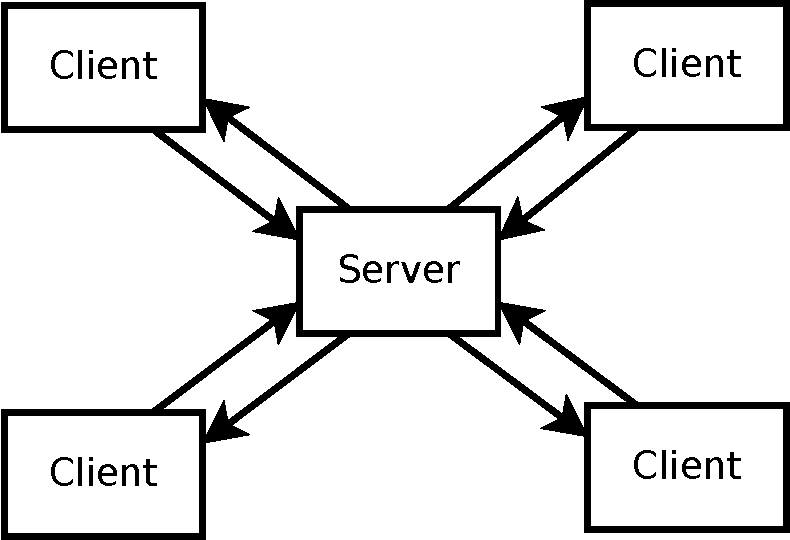
\includegraphics[width=0.44\linewidth]{../images/client-server-model-crop.pdf} &
		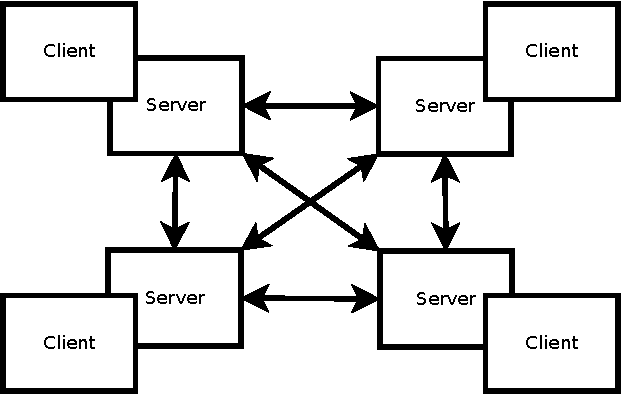
\includegraphics[width=0.48\linewidth]{../images/client-distributed-server-model-crop.pdf} \\
		(a) & (b)
	\end{tabular}

	\caption{\label{figure:server-models} The first model (a) is a \clientServer model. In this model all of the clients send updates to the server and the server send updates out to the clients. In the second model (b) the server is distributed and clients communicate with many servers.}
	\end{figure}
	
	\subsubsection{Protocol and Messaging}
	
	The clients send updates/events to every server. For \fire{\agent_{i}}{\agent_{j}} events the server that is paired with the client with $\agent_{j}$ will determine the outcome. If the \fire{\agent_{i}}{\agent_{j}} event is successful according to the authoritative server a \destroy{\agent_{j}} event is broadcast to every server. All communication is asynchronous except for the \destroy{\agent_{j}} event that will need to be acknowledged by each server.

